\section{Evaluation}
So far, we have presented a procedure and automated compo\-nent-based framework for extracting the performance properties of generated code. In this section, we evaluate the implementation of our approach by explaining the design of our empirical study and the different methods we used to assess the effectiveness of our approach. 
The experimental material is available for replication purposes\footnote{\url{https://testingcodegenerators.wordpress.com/}}.
\subsection{Experimental Setup}
\subsubsection{Code Generators Under Test: Haxe compilers}
In order to test the applicability of our approach, we conduct experiments on a popular high-level programming language called Haxe and its code generators. 
%Haxe is an open source toolkit for cross-platform development which compiles to a number of different programming platforms, including JavaScript, Flash, PHP, C++, C\# and Java. Haxe involves many features: the Haxe language, multi-platform compilers, and different native libraries. 
%The Haxe language is a high-level programming language which is strictly typed. This language supports both functional programming and object-oriented programming paradigms. It has a common type hierarchy, making certain API available on every targeted platform.
Haxe comes with a set of compilers that translate manually-written code (in Haxe language) to different target languages and platforms. 
%Haxe code can be compiled for applications running on desktop, mobile and web platforms. Compilers ensure the correctness of user code in terms of syntax and type safety.
%Haxe comes also with a set of standard libraries that can be used on all supported targets and platform-specific libraries for each of them.

The process of code transformation and generation can be described as following: Haxe compilers analyzes the source code written in Haxe language then, the code is checked and parsed into a typed structure, resulting in a typed abstract syntax tree (AST). This AST is optimized and transformed afterwards to produce source code for target platform/language.

Haxe offers the option of choosing which platform to target for each program using a command-line tool. Moreover, some optimizations and debugging information can be enabled through CLI but in our experiments, we did not turned on any further options. 

\subsubsection{Cross-platform Benchmark}
One way to prove the effectiveness of our approach is to create benchmarks. Thus, we use the Haxe language and its code generators to build a cross-platform benchmark. The proposed benchmark is composed of a collection of cross-platform libraries that can be compiled to different targets. In these experiments, we consider five Haxe code generators to test: Java, JS, C++, CS, and PHP code generators. To select cross-platform libraries, we explore github and we use the Haxe library repository\footnote{\url{http://thx-lib.org/}}. We select seven libraries that have the best code coverage score. 

In fact, each Haxe library comes with an API and a set of test suites. These tests, written in Haxe, represent a set of unit tests that covers the different functions of the API. The main task of these tests is to check the correct functional behavior of generated programs once generated code is executed within the target platform. To prepare our benchmark, we remove all the tests that fail to compile to our five targets (i.e., errors, crashes and failures) and we keep only test suites that are functionally correct in order to focus only on the non-functional properties.

Moreover, we add manually new test cases to some libraries in order to extend the number of test suites. The number of test suites depends on the number of existing functions within the Haxe library.



We use then, these test suites then, to generate a load and stress the target library. This can be useful to study the impact of this load on the resource usage of the system. For example, if one test suite consumes a lot of resources for a specific target, then this could be explained by the fact that the code generator has produced code that is very greedy in terms of resources.

Thus, we run each test suite 1000 times to get comparable values in terms of resource usage.
Table 2 describes the Haxe libraries that we have selected in this benchmark to evaluate our
approach.

\begin{table}[h]
	\centering

	\begin{tabular}{|c|c|p{4.3cm}|}
		\hline
		\textbf{Library} & \textbf{\#TestSuites} & \textbf{Description} \\
		\hline
		Color  &  19 &  Color conversion from/to any color space   \\ \hline
		Core & 51  & Provides extensions to many types  \\ \hline
		Hxmath & 6  & A 2D/3D math library  \\ \hline
	    Format  &  4 & Format library such as dates, number formats   \\ \hline
		Promise & 3  & Library for lightweight promises and futures  \\ \hline
		Culture & 4  & Localization library for Haxe \\ \hline
		Math & 3  & Generation of random values \\ \hline
	\end{tabular}
		\caption{Description of selected benchmark libraries}
		\label{my-label}
\end{table}

\subsubsection{Evaluation Metrics Used}
We use to evaluate the efficiency of generated code using the following non-functional metrics:

-\textit{Memory usage}:
It corresponds to the maximum memory consumption of the running container under test. Memory usage is measured in Mbytes.

-\textit{Execution time}:
Program execution time is measured in seconds.

We recall that our tool is able to evaluate other non-functional properties of generated code such as code generation time, compilation time, code size, CPU usage. We choose to focus, in this experiment, on the performance (i.e., execution time) and resource usage (i.e., memory usage).
 
\subsubsection{Setting up Infrastructure}
\begin{figure}[h]
	\centering
	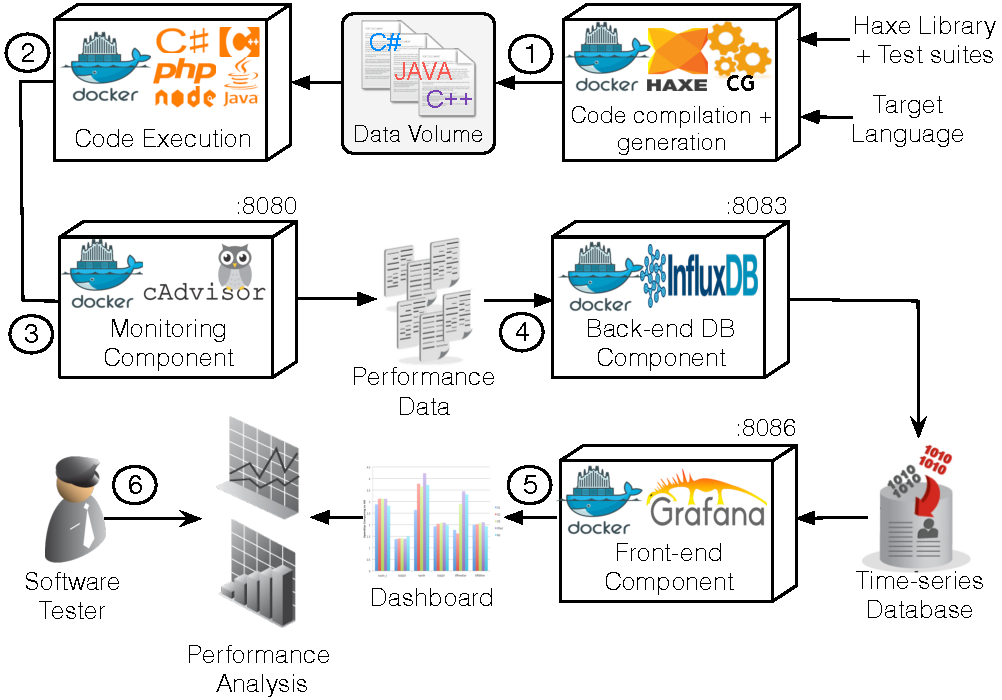
\includegraphics[width=1\linewidth]{Ressources/settingup.pdf}
	\caption{Infrastructure settings for running experiments}
\end{figure}
To assess our approach, we configure our previously proposed container-based infrastructure in order to run experiments on the Haxe case study.
Figure 3 shows a big picture of the testing and monitoring infrastructure considered in these experiments.


\begin{table}[h]
	\centering

	\resizebox{\columnwidth}{!}{%
	\begin{tabular}{|l|l|S[table-format=3.2]|l|S[table-format=3.2]|l|S[table-format=3.2]|}
		\hline
		\textbf{Benchmark}                 & \textbf{TestSuite} & \textbf{Std\_dev}                & \textbf{TestSuite} & \textbf{Std\_dev}             & \textbf{TestSuite} & \textbf{Std\_dev}              \\ \hline
		& \textbf{TS1}       & 0.55                             & \textbf{TS8}       & 0.24                          & \textbf{TS15}      & 0.73                           \\ \cline{2-7} 
		& \textbf{TS2}       & 0.29                             & \textbf{TS9}       & 0.22                          & \textbf{TS16}      & 0.12                           \\ \cline{2-7} 
		& \textbf{TS3}       & 0.34                             & \textbf{TS10}      & 0.10                          & \textbf{TS17}      & 0.31                           \\ \cline{2-7} 
		& \textbf{TS4}       & 2.51                             & \textbf{TS11}      & 0.17                          & \textbf{TS18}      & 0.34                           \\ \cline{2-7} 
		& \textbf{TS5}       & 1.53                             & \textbf{TS12}      & 0.28                          & \textbf{TS19}      & \cellcolor[HTML]{C0C0C0}120.61 \\ \cline{2-7} 
		& \textbf{TS6}       & 43.50                            & \textbf{TS13}      & 0.33                         & \multicolumn{2}{l|}{\multirow{2}{*}{}} \\ \cline{2-5}
		\multirow{-7}{*}{\textbf{Color}}   & \textbf{TS7}       & 0.50                             & \textbf{TS14}      & 1.88                          & \multicolumn{2}{l|}{}                  \\ \hline
		& \textbf{TS1}       & 0.35                             & \textbf{TS18}      & 0.16                          & \textbf{TS35}      & 1.30                           \\ \cline{2-7} 
		& \textbf{TS2}       & 0.07                             & \textbf{TS19}      & 0.60                          & \textbf{TS36}      & 1.13                           \\ \cline{2-7} 
		& \textbf{TS3}       & 0.30                             & \textbf{TS20}      & 5.79                          & \textbf{TS37}      & 2.02                           \\ \cline{2-7} 
		& \textbf{TS4}       & \cellcolor[HTML]{C0C0C0}27299.89 & \textbf{TS21}      & 0.47                          & \textbf{TS38}      & 0.26                           \\ \cline{2-7} 
		& \textbf{TS5}       & 6.12                             & \textbf{TS22}      & 2.74                          & \textbf{TS39}      & 0.16                           \\ \cline{2-7} 
		& \textbf{TS6}       & 21.90                            & \textbf{TS23}      & 2.14                          & \textbf{TS40}      & 8.12                           \\ \cline{2-7} 
		& \textbf{TS7}       & 0.41                             & \textbf{TS24}      & 3.79                          & \textbf{TS41}      & 5.45                           \\ \cline{2-7} 
		& \textbf{TS8}       & 0.28                             & \textbf{TS25}      & 0.19                          & \textbf{TS42}      & 0.11                           \\ \cline{2-7} 
		& \textbf{TS9}       & 0.78                             & \textbf{TS26}      & 0.13                          & \textbf{TS43}      & 1.41                           \\ \cline{2-7} 
		& \textbf{TS10}      & 1.82                             & \textbf{TS27}      & 5.59                          & \textbf{TS44}      & 1.56                           \\ \cline{2-7} 
		& \textbf{TS11}      & \cellcolor[HTML]{C0C0C0}180.68   & \textbf{TS28}      & 1.71                          & \textbf{TS45}      & 0.11                           \\ \cline{2-7} 
		& \textbf{TS12}      & \cellcolor[HTML]{C0C0C0}185.02   & \textbf{TS29}      & 0.26                          & \textbf{TS46}      & 1.04                           \\ \cline{2-7} 
		& \textbf{TS13}      & \cellcolor[HTML]{C0C0C0}128.78   & \textbf{TS30}      & 0.44                          & \textbf{TS47}      & 0.23                           \\ \cline{2-7} 
		& \textbf{TS14}      & 0.71                             & \textbf{TS31}      & 1.71                          & \textbf{TS48}      & 1.34                           \\ \cline{2-7} 
		& \textbf{TS15}      & 0.12                             & \textbf{TS32}      & 2.42                          & \textbf{TS49}      & 1.86                           \\ \cline{2-7} 
		& \textbf{TS16}      & 0.65                             & \textbf{TS33}      & 8.29                          & \textbf{TS50}      & 1.28                           \\ \cline{2-7} 
		\multirow{-17}{*}{\textbf{Core}}   & \textbf{TS17}      & 0.26                             & \textbf{TS34}      & 5.25                          & \textbf{TS51}      & 3.53                           \\ \hline
		& \textbf{TS1}       & 31.65                            & \textbf{TS3}       & 30.34                         & \textbf{TS5}       & 0.40                           \\ \cline{2-7} 
		\multirow{-2}{*}{\textbf{Hxmath}}  & \textbf{TS2}       & 4.27                             & \textbf{TS4}       & 0.25                          & \textbf{TS6}       & 0.87                           \\ \hline
		& \textbf{TS1}       & 0.28                             & \textbf{TS3}       & \cellcolor[HTML]{C0C0C0}95.36 & \textbf{TS4}       & 1.49                           \\ \cline{2-7} 
		\multirow{-2}{*}{\textbf{Format}}  & \textbf{TS2}       & \cellcolor[HTML]{C0C0C0}64.94    & \multicolumn{4}{l|}{\textbf{}}                                                                           \\ \hline
		\textbf{Promise}                   & \textbf{TS1}       & 0.29                             & \textbf{TS2}       & 13.21                         & \textbf{TS3}       & 1.21                           \\ \hline
		& \textbf{TS1}       & 0.13                             & \textbf{TS3}       & 0.13                          & \textbf{TS4}       & 1.40                           \\ \cline{2-7} 
		\multirow{-2}{*}{\textbf{Culture}} & \textbf{TS2}       & 0.10                             & \multicolumn{4}{l|}{}                                                                                    \\ \hline
		\textbf{Math}                      & \textbf{TS1}       & \cellcolor[HTML]{C0C0C0}642.85   & \textbf{TS2}       & 28.32                         & \textbf{TS3}       & 24.40                          \\ \hline
	\end{tabular}%
	}
 
		\caption{The comparison results of running each test suite across five target languages: the metric used is the standard deviation between execution times  }
 
 
 
		\label{my-label}
\end{table}

% Please add the following required packages to your document preamble:
% \usepackage{multirow}
% Please add the following required packages to your document preamble:
% \usepackage{multirow}
% \usepackage[table,xcdraw]{xcolor}
% If you use beamer only pass "xcolor=table" option, i.e. \documentclass[xcolor=table]{beamer}
\begin{table}[]
	\centering

	\resizebox{\columnwidth}{!}{%
	\begin{tabular}{|l|l|S[table-format=3.2]|l|S[table-format=3.2]|l|S[table-format=3.2]|}
		\hline
		\textbf{Benchmark}                 & \textbf{TestSuite} & \textbf{Std\_dev}               & \textbf{TestSuite} & \textbf{Std\_dev}              & \textbf{TestSuite} & \textbf{Std\_dev}              \\ \hline
		& \textbf{TS1}       & 10.19                           & \textbf{TS8}       & 1.23                           & \textbf{TS15}      & 14.44                          \\ \cline{2-7} 
		& \textbf{TS2}       & 1.17                            & \textbf{TS9}       & 1.95                           & \textbf{TS16}      & 1.13                           \\ \cline{2-7} 
		& \textbf{TS3}       & 0.89                            & \textbf{TS10}      & 1.27                           & \textbf{TS17}      & 0.72                           \\ \cline{2-7} 
		& \textbf{TS4}       & 30.34                           & \textbf{TS11}      & 0.57                           & \textbf{TS18}      & 0.97                           \\ \cline{2-7} 
		& \textbf{TS5}       & 31.79                           & \textbf{TS12}      & 1.11                           & \textbf{TS19}      & \cellcolor[HTML]{C0C0C0}777.32 \\ \cline{2-7} 
		& \textbf{TS6}       & \cellcolor[HTML]{C0C0C0}593.05  & \textbf{TS13}      & 0.46                           & \multicolumn{2}{l|}{}                               \\ \cline{2-5}
		\multirow{-7}{*}{\textbf{Color}}   & \textbf{TS7}       & 12.14                           & \textbf{TS14}      & 45.90                          & \multicolumn{2}{l|}{\multirow{-2}{*}{}}             \\ \hline
		& \textbf{TS1}       & 1.40                            & \textbf{TS18}      & 1.00                           & \textbf{TS35}      & 14.13                          \\ \cline{2-7} 
		& \textbf{TS2}       & 1.17                            & \textbf{TS19}      & 20.37                          & \textbf{TS36}      & 32.41                          \\ \cline{2-7} 
		& \textbf{TS3}       & 0.60                            & \textbf{TS20}      & 128.23                         & \textbf{TS37}      & 22.72                          \\ \cline{2-7} 
		& \textbf{TS4}       & \cellcolor[HTML]{C0C0C0}403.15  & \textbf{TS21}      & 24.38                          & \textbf{TS38}      & 2.19                           \\ \cline{2-7} 
		& \textbf{TS5}       & 41.95                           & \textbf{TS22}      & 76.24                          & \textbf{TS39}      & 0.26                           \\ \cline{2-7} 
		& \textbf{TS6}       & 203.55                          & \textbf{TS23}      & 18.82                          & \textbf{TS40}      & 126.29                         \\ \cline{2-7} 
		& \textbf{TS7}       & 19.69                           & \textbf{TS24}      & 72.01                          & \textbf{TS41}      & 31.01                          \\ \cline{2-7} 
		& \textbf{TS8}       & 0.78                            & \textbf{TS25}      & 0.21                           & \textbf{TS42}      & 0.93                           \\ \cline{2-7} 
		& \textbf{TS9}       & 30.41                           & \textbf{TS26}      & 2.30                           & \textbf{TS43}      & 50.36                          \\ \cline{2-7} 
		& \textbf{TS10}      & 57.19                           & \textbf{TS27}      & 101.53                         & \textbf{TS44}      & 12.56                          \\ \cline{2-7} 
		& \textbf{TS11}      & 68.92                           & \textbf{TS28}      & 43.67                          & \textbf{TS45}      & 0.91                           \\ \cline{2-7} 
		& \textbf{TS12}      & 74.19                           & TS29               & 0.90                           & \textbf{TS46}      & 27.28                          \\ \cline{2-7} 
		& \textbf{TS13}      & 263.99                          & \textbf{TS30}      & 4.02                           & \textbf{TS47}      & 1.10                           \\ \cline{2-7} 
		& \textbf{TS14}      & 19.89                           & \textbf{TS31}      & 52.35                          & \textbf{TS48}      & 15.40                          \\ \cline{2-7} 
		& \textbf{TS15}      & 0.30                            & \textbf{TS32}      & 134.75                         & \textbf{TS49}      & 37.01                          \\ \cline{2-7} 
		& \textbf{TS16}      & 28.29                           & \textbf{TS33}      & 82.66                          & \textbf{TS50}      & 23.29                          \\ \cline{2-7} 
		\multirow{-17}{*}{\textbf{Core}}            & \textbf{TS17}      & 1.16                            & \textbf{TS34}      & 89.57                          & \textbf{TS51}      & 1.28                           \\ \hline
		& \textbf{TS1}       & \cellcolor[HTML]{C0C0C0}444.18  & \textbf{TS3}       & \cellcolor[HTML]{C0C0C0}425.65 & \textbf{TS5}       & 17.69                          \\ \cline{2-7} 
		\multirow{-2}{*}{\textbf{Hxmath}}  & \textbf{TS2}       & 154.80                          & \textbf{TS4}       & 0.96                           & \textbf{TS6}       & 46.13                          \\ \hline
		& \textbf{TS1}       & 0.74                            & \textbf{TS3}       & 255.36                         & \textbf{TS4}       & 8.40                           \\ \cline{2-7} 
		\multirow{-2}{*}{\textbf{Format}}  & \textbf{TS2}       & 106.87                          & \multicolumn{4}{l|}{\textbf{}}                                                                            \\ \hline
		\textbf{Promise}                   & \textbf{TS1}       & 0.30                            & \textbf{TS2}       & 58.76                          & \textbf{TS3}       & 20.04                          \\ \hline
		& \textbf{TS1}       & 1.28                            & \textbf{TS3}       & 0.58                           & \textbf{TS4}       & 15.69                          \\ \cline{2-7} 
		\multirow{-2}{*}{\textbf{Culture}} & \textbf{TS2}       & 4.51                            & \multicolumn{4}{l|}{}                                                                                     \\ \hline
		\textbf{Math}                      & \textbf{TS1}       & \cellcolor[HTML]{C0C0C0}1041.53 & \textbf{TS2}       & 234.93                         & \textbf{TS3}       & 281.12                         \\ \hline
	\end{tabular}%
}
 
	\caption{The comparison results of running each test suite across five target languages: the metric used is the standard deviation between memory consumptions}
 
 

	\label{my-label}
\end{table}



\begin{table*}[h]
	\centering
	
	\resizebox{0.75\linewidth}{!}{%
		\begin{tabular}{|l|S[table-format=3.2]|S[table-format=3.2]|S[table-format=3.2]|S[table-format=3.2]|S[table-format=3.2]|S[table-format=3.2]|S[table-format=3.2]|S[table-format=3.2]|S[table-format=3.2]|S[table-format=3.2]|}
			\hline
			\multirow{2}{*}{}    & \multicolumn{2}{c|}{\textbf{JS}}   & \multicolumn{2}{c|}{\textbf{JAVA}} & \multicolumn{2}{c|}{\textbf{C++}}  & \multicolumn{2}{c|}{\textbf{CS}}   & \multicolumn{2}{c|}{\textbf{PHP}}  \\ \cline{2-11} 
			& \textbf{Time} & \textbf{Factor} & \textbf{Time} & \textbf{Factor} & \textbf{Time} & \textbf{Factor} & \textbf{Time} & \textbf{Factor} & \textbf{Time} & \textbf{Factor} \\ \hline
			\textbf{Color\_TS19} & 4.52             & x1.0            & 8.61             & x1.9            & 10.73            & x2.4            & 14.99            & x3.3            & 279.27           & x61.8           \\ \hline
			\textbf{Core\_TS4}   & 665.78           & x1.0            & 416.85           & x0.6            & 699.11           & x1.1            & 1161.29          & x1.7            & 61777.21         & x92.8           \\ \hline
			\textbf{Core\_TS11}  & 4.27             & x1.0            & 1.80             & x0.4            & 1.57             & x0.4            & 5.71             & x1.3            & 407.33           & x95.4           \\ \hline
			\textbf{Core\_TS12}  & 4.71             & x1.0            & 2.06             & x0.4            & 1.60             & x0.3            & 5.36             & x1.1            & 417.14           & x88.6           \\ \hline
			\textbf{Core\_TS13}  & 6.26             & x1.0            & 5.91             & x0.9            & 11.04            & x1.8            & 14.14            & x2.3            & 297.21           & x47.5           \\ \hline
			\textbf{Format\_TS2}   & 2.31             & x1.0            & 2.10             & x0.9            & 1.81             & x0.8            & 6.08             & x2.6            & 148.24           & x64.1           \\ \hline
			\textbf{Format\_TS3}   & 5.40             & x1.0            & 5.03             & x0.9            & 7.67             & x1.4            & 12.38            & x2.3            & 220.76           & x40.9           \\ \hline
			\textbf{Math\_TS1}   & 3.01             & x1.0            & 12.51            & x4.2            & 16.30            & x5.4            & 14.14            & x4.7            & 1448.90          & x481.7          \\ \hline
		\end{tabular}%
	}
	\caption{Raw data values of test suites that led to the highest variation in terms of execution time}
	\label{my-label}
\end{table*}


\begin{table*}[h]
	\centering

	\resizebox{0.75\linewidth}{!}{%
	\begin{tabular}{|l|S[table-format=3.2]|S[table-format=3.2]|S[table-format=3.2]|S[table-format=3.2]|S[table-format=3.2]|S[table-format=3.2]|S[table-format=3.2]|S[table-format=3.2]|S[table-format=3.2]|S[table-format=3.2]|}
		\hline
		\multirow{2}{*}{}    & \multicolumn{2}{c|}{\textbf{JS}}      & \multicolumn{2}{c|}{\textbf{JAVA}}    & \multicolumn{2}{c|}{\textbf{C++}}     & \multicolumn{2}{c|}{\textbf{CS}}      & \multicolumn{2}{c|}{\textbf{PHP}}     \\ \cline{2-11} 
		& \textbf{Memory} & \textbf{Factor} & \textbf{Memory} & \textbf{Factor} & \textbf{Memory} & \textbf{Factor} & \textbf{Memory} & \textbf{Factor} & \textbf{Memory} & \textbf{Factor} \\ \hline
		\textbf{Color\_TS6}  & 900.70              & x1.0            & 1362.55              & x1.5            & 2275.49             & x2.5            & 1283.31             & x1.4            & 758.79              & x0.8            \\ \hline
		\textbf{Color\_TS19} & 253.01              & x1.0            & 819.92              & x3.2            & 923.99              & x3.7            & 327.61              & x1.3            & 2189.86             & x8.7            \\ \hline
		\textbf{Core\_TS4}   & 303.09              & x1.0            & 768.22              & x2.5            & 618.42              & x2              & 235.75              & x0.8            & 1237.15             & x4.1            \\ \hline
		\textbf{Hxmath\_TS1} & 104.00              & x1.0            & 335.50              & x3.2            & 296.43              & x2.9            & 156.41              & x1.5            & 1192.98             & x11.5           \\ \hline
		\textbf{Hxmath\_TS3} & 111.68              & x1.0            & 389.73              & x3.5            & 273.12              & x2.4            & 136.49              & x1.2            & 1146.05             & x10.3           \\ \hline
		\textbf{Math\_TS1}   & 493.66              & x1.0            & 831.44              & x1.7            & 1492.97             & x3              & 806.33              & x1.6            & 3088.15             & x6.3            \\ \hline
	\end{tabular}%
}
	\caption{Raw data values of test suites that led to the highest variation in terms of memory usage}
	\label{my-label}
\end{table*}

 

First, we create a new Docker image in where we install the Haxe code generators and compilers (through the configuration file "Dockerfile"). Then a new instance of that image is created. It takes as an input the Haxe library we would to test and the list of test suites (step 1). It produces as an output the source code and binaries that have to be executed. These files are saved in a shared repository.
In Docker environment, this repository is called "data volume". A data volume is a specially-designated directory within containers that shares data with the host machine. So, when
we execute the generated test suites, we provide a shared volume with
the host machine so that, binaries can be executed in the execution container (Step 2). In fact, for the code execution we created, as well, a new Docker image in where we install all execution tools and environments such as php interpreter, NodeJS, etc. 

In the meantime, while running test suites inside the container, we collect runtime resource usage data using cAdvisor (step 3). The cAdvisor Docker image does not need any configuration on the host machine. We have just to run it on our host machine. It will then have access to resource usage and performance characteristics of all running containers. This image uses the Cgroups mechanism described previously to collect, aggregate, process, and export ephemeral real-time information about running containers. Then, it reports all statistics via web UI to view live resource consumption of each container. cAdvisor has been widely used in different projects such as Heapster\footnote{\url{https://github.com/kubernetes/heapster}} and Google Cloud Platform\footnote{\url{https://cloud.google.com/}}. In this experiment, we choose to gather information about the memory usage of running container.
Afterwards, we record these data into a new time-series database using our InfluxDB back-end container (step 4). %Thus, we define its corresponding ip port into the monitoring component so that, container statistics are sent over TCP port (e.g., \textit{8083}) exposed by the database component. 

Next, we run Grafana and we link it to InfluxDB. % by setting up the data source port 8086 so that, 
Grafana can  request data from the database. We recall that InfluxDB also provides a web UI to query the database and show graphs (step 5). But, Grafana let us display live results over time in much pretty looking graphs. Same as InfluxDB, we use SQL queries to extract non-functional metrics from the database for visualization and analysis (step 6). In our experiment, we are gathering the maximum memory usage values without presenting the graphs of resource usage profiles.

To obtain comparable and reproducible results, we use the same hardware across all experiments: a farm of AMD A10-7700K APU Radeon(TM) R7 Graphics processor with 4 CPU cores (\SI{2.0}{\GHz}), running Linux with a 64 bit kernel and \SI{16}{\giga\byte} of system memory. We reserve one core and \SI{4}{\giga\byte} of memory for each running container. 

\subsection{Experimental Results}
\subsubsection{Evaluation using the standard deviation}
We now conduct experiments based on the Haxe benchmark. We run each test suite 1K times and we report the execution time and memory usage across the different target languages: Java, JS, C++, CS, and PHP. 
The goal of running these experiments is to observe and compare the behavior of generated code regarding the testing load. We recall, as mentioned in the motivation, that we are not using any oracle function to detect inconsistencies. However, we rely on the comparison results across different targets to define code generator inconsistencies.
Thus, we use, as a quality metric, the standard deviation to quantify the amount of variation among execution traces (i.e., memory usage or execution time) and that for the five target languages. We recall that the formula of standard deviation is the square root of the variance. Thus, we are calculating this variance as the squared differences from the mean. Our data values in our experiment represent the obtained values in five languages. So, for each test suite we are taking the mean of these five values in order to calculate the variance.
A low standard deviation of a test suite execution, indicates that the data points (execution time or memory usage data) tend to be close to the mean which we consider as an acceptable behavior.  
On the other hand, a high standard deviation indicates that one or more data points are spread out over a wider range of values which can be more likely interpreted as a code generator inconsistency. 



In Table 3, we report the comparison results of running the benchmark in terms of execution speed. At the first glance, we can clearly see that all standard deviations are more mostly close to 0 - 8 interval. It is completely normal to get such small deviations, because we are comparing the execution time of test suites that are written in heterogeneous languages and executed using different technologies (e.g., interpreters for PHP, JVM for JAVA, etc.). So, it is expected to get a small deviation between the execution times after running the test suite in different languages. However, we remark in the same table, that there are some variation points where the deviation is relatively high. We count 8 test suites where the deviation is higher than 60 (highlighted in gray). We choose this value (i.e., standard deviation = 60) as a threshold to designate the points where the variation is extremely high. Thus, we consider values higher than 60 as a potential possibility that a non-functional bug could occur. These variations can be explained by the fact that the execution speed of one or more test suites varies considerably from one language to another. This argues the idea that the code generator has produced a suspect behavior of code for one or more target language. We provide later better explanation in order to detect the faulty code generators.

Similarly, Table 4 resumes the comparison results of test suites execution regarding memory usage. The variation in this experiment are more important than previous results. This can be argued by the fact that the memory utilization and allocation patterns are different for each language. Nevertheless, we can recognize some points where the variation is extremely high. Thus, we choose a threshold value equal to 400 and we highlighted, in gray, the points that exceed this threshold. Thus, we detect 6 test suites where the variation is extremely high. 
One of the reasons that caused this variation may occur when the test suite executes some parts of the code (in a specific language) that are so greedy in terms of resources. This may be not the case when the variation is lower than 10 for example.
We assume then that the faulty code generator, in this case, represents a threat for software quality since it can generate a code that is very resource consuming.
 
The inconsistencies we are trying to find here are more related to the incorrect memory utilization patterns produced by the faulty code generator. Such inconsistencies may come from an inadequate type usage, high resource instantiation, etc.





\subsubsection{Analysis}
Now that we have observed the non-functional behavior of test suites execution in different languages, we can analyze the extreme points we have detected in previous tables to observe more in deep the source of such deviation.
For that reason, we present in Table 5 and 6 the raw data values of these extreme test suites in terms of execution time and memory usage. 

Table 5 is showing the execution time of each test suite in a specific target language. We provide also factors of execution times among test suites running in different languages by taking as a baseline the JS version. 
We can clearly see that the PHP code has can have a singular behavior regarding the performance with a factor ranging from x40.9 for test suite 3 in benchamrk Format (Format\_TS3) to x481.7 for Math\_TS1. We remark also that running Core\_TS4 takes 61777 seconds (almost 17 hours) compared to a 416 seconds (around 6 minutes) in JAVA which is a very large gap. The highest factor detected for other languages ranges from x0.3 to x5.4 which is not negligible but it represents a small deviation compared to PHP version. While it is true that we are comparing different versions of generated code, it was expected to get some variations while running test cases in terms of execution time. However, in the case of PHP code generator it is far to be a simple variation but it is more likely to be a code generator inconsistency that led to such performance regression.


Meanwhile, we gathered information about the points that led to the highest standard deviation in terms of memory usage. Table~6 shows these results. %We take as well the JS version as a baseline since it requires less memory. 
Again, we can identify singular behavior regarding the performance. For Color\_TS6, C\# version consumes the highest memory (x2.5 more than JS). For other test suites versions, the factor varies from x0.8 to x3.7. %Besides the performance issues of PHP code generator presented in table~5, the results of memory usage confirm our claim since the PHP code has the highest memory utilization.
 
Focusing particularly on the singular performance of PHP code in core TS4, we observe the intensive use of \textit{"arrays"} in most of the functions under test. Arrays are known to be slow in PHP and PHP library has introduced many advanced functions such as $array\_fill$ and specialized abstract types such as \textit{"SplFixedArray"}\footnote{\url{http://php.net/manual/fr/class.splfixedarray.php}} to overcome this limitation. By changing just these two parts in the code generator, we improve the PHP code speed with a factor x5. 


In short, the lack of use of specific types, in native PHP standard library, by the PHP code generator such as \textit{SplFixedArray} shows a real impact on the non-functional behavior of generated code. In contrast, selecting carefully the adequate types and functions to generate code by code generators can lead to performance improvement.  We can observe the same kind of error in the C++ program  during one test suite execution (Color\_TS6) which consumes too much memory. The types used in the code generator are not the best ones. 

\subsection{Threats to Validity}
Any automated approach has limitations. We resume, in the following paragraphs, external and internal threats that can be raised:

\textit{External validity} refers to the generalizability of our findings. In this study, we perform experiments on Haxe and a set of test suite selected from Github and from the Haxe community. We have no guarantee that these libraries covers all the Haxe language features neither than all the Haxe standard libraries. Consequently, we cannot guarantee that the approach is able to find all the code generators issues. In particular, the threshold to detect singular behavior has a huge impact on the precision and recall of the proposed approach. Experiments should be replicated to other case studies to confirm our findings and try to understand the best heuristic to detect the code generator issues regarding performance. 

\textit{Internal validity} is concerned with the use of a container-based approach. Even if it exists emulator such as Qemu that allows to reflect the behavior of heterogeneous hardware, the chosen infrastructure has not been evaluated to test generated code that target heterogeneous hardware machine. In such a case, the provided compiler for a dedicated hardware can provide specific optimizations that lead to a large number of false positives. 
 


%hrough these conducted experiments, we reached interesting results, some of which were unexpected.


%In most languages, arrays are fixed-sized, but this is not the case in PHP since they are allocated dynamically. The dynamic allocation of arrays  leads to a slower write time because the memory locations needed to hold the new data is not already allocated. Thus, slow writing speed damages the performance of PHP code and impact the memory usage. This observation clearly confirm our early findings. The solution for this problem may be to use another type of object from the Standard PHP Library. As an alternative, \textit{"SplFixedArray"} pre-allocates the necessary memory and allows a faster array implementation, thereby solving the issue of slower write times. [ref to spl benchs]

%\subsection{Discussions}
%For instance, the poor performance of the Haxe-produced PHP code was certainly a surprise. 
%The PHP target had a very large execution time and memory usage for almost every test suite execution. 
%That is to say that PHP code generator is clearly generating non-efficient code regarding the non-functional properties. It is even possible to say that other code generators are not extremely efficient since we found that C++ code consumed, during one test suite execution (Color\_TS6), more memory than PHP. But, we cannot say for sure that C++ code generator is buggy. Thus, we cannot make any assumption. Nevertheless, the only point which, at this stage, can be statistically made is that PHP code generator has a real performance issue that has to be fixed by code generators developers. 

%In attempting to understand the reasons of this PHP performance issues, we tried to take a look at the source code generated in PHP. As an example, we looked at the source code of Core\_TS4. 





 






